% Inbuilt themes in beamer
\documentclass{beamer}

% Theme choice:
\usetheme{CambridgeUS}
\graphicspath{{figure/}}

% Title page details: 
\title{Assignment-2} 
\author{CS21BTECH11056}
\date{\today}
\logo{\large \LaTeX{}}


\begin{document}

% Title page frame
\begin{frame}
    \titlepage 
\end{frame}

% Remove logo from the next slides
\logo{}


% Outline frame
\begin{frame}{Question}
    \tableofcontents
    Question 20(b)\\
	From the given data :\\

\begin{table}[h!]
\center
%\resizebox{\columnwidth}{!}
{
\begin{tabular}{|c|c|c|}
\hline
Variable & x & y\\
\hline
Mean & 6 & 8\\
\hline
 Standard Deviation & 4 & 6\\
 \hline
\end{tabular}
}
\end{table}
and correlation coefficient : $\frac{2}{3}$  Find :\\
(i)	 Regression coefficient $ b_{yx} $ and $b_{xy}$\\
(ii) Regression line x on y\\
(ii) Most likely value of x when y = 14\\

\end{frame}


% Lists frame
\begin{frame}{Solution :}
$\bar{x}$ = 6 , $\bar{y}$ = 8\\
$\sigma_{x}$ = 4 , $\sigma_{y}$ = 6\\ 
r = $\frac{2}{3}$\\
\begin{align}
b_{yx} &= r.\frac{\sigma_{y}}{\sigma_{x}}
        = \frac{2}{3}.\frac{6}{4}
        = 1\\
b_{xy} &= r.\frac{\sigma_{x}}{\sigma_{y}}
        = \frac{2}{3}.\frac{4}{6}
        = \frac{4}{9}
\end{align}

\end{frame}

\begin{frame}
Regression equation x on y\\
\begin{align*}
x - \bar{x} &= bxy( y -\bar{y} )\\
x - 6       &= \frac{4}{9} ( y - 8)\\
9x - 54     &= 4y - 32\\
9x - 4y     &= 22
\end{align*}
    When y = 14 ,
\begin{align*}
(9x - 4) 14 &= 22\\
         9x &= 78\\
          x &= 8.67
\end{align*}
\end{frame} 

\begin{frame}{Graph :}

\begin{figure}[h!]
\centering
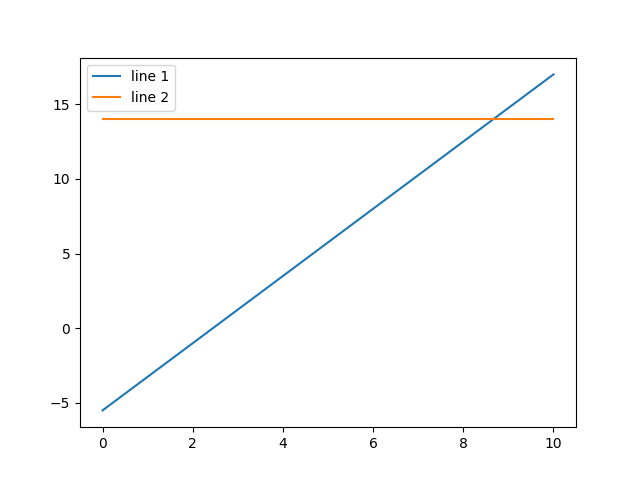
\includegraphics[width= 8 cm]{fig1.png}
\caption{Finding the intersection point}
\label{Fig1}
\end{figure}

\end{frame}

\end{document}